\documentclass{standalone}
\usepackage{tikz}
\usepackage{tikz-cd}
\usepackage{tikz-3dplot}
\usepackage{pgfplots}
\usepackage{pgffor} % For \foreach loop
\pgfplotsset{compat=newest} % Adjust to your version of pgfplots
\def\Circlearrowleft{\ensuremath{%
		\rotatebox[origin=c]{180}{$\circlearrowleft$}}}
\def\Circlearrowright{\ensuremath{%
		\rotatebox[origin=c]{180}{$\circlearrowright$}}}
\def\CircleArrowleft{\ensuremath{%
		\reflectbox{\rotatebox[origin=c]{180}{$\circlearrowleft$}}}}
\def\CircleArrowright{\ensuremath{%
		\reflectbox{\rotatebox[origin=c]{180}{$\circlearrowright$}}}}
\usetikzlibrary{
	3d, % For 3D drawing
	angles,
	arrows,
	arrows.meta,
	backgrounds,
	bending,
	calc,
	decorations.pathmorphing,
	decorations.pathreplacing,
	decorations.markings,
	fit,
	matrix,
	patterns,
	patterns.meta,
	positioning,
	quotes,
	shadows,
	shapes,
	shapes.geometric
}

\begin{document}
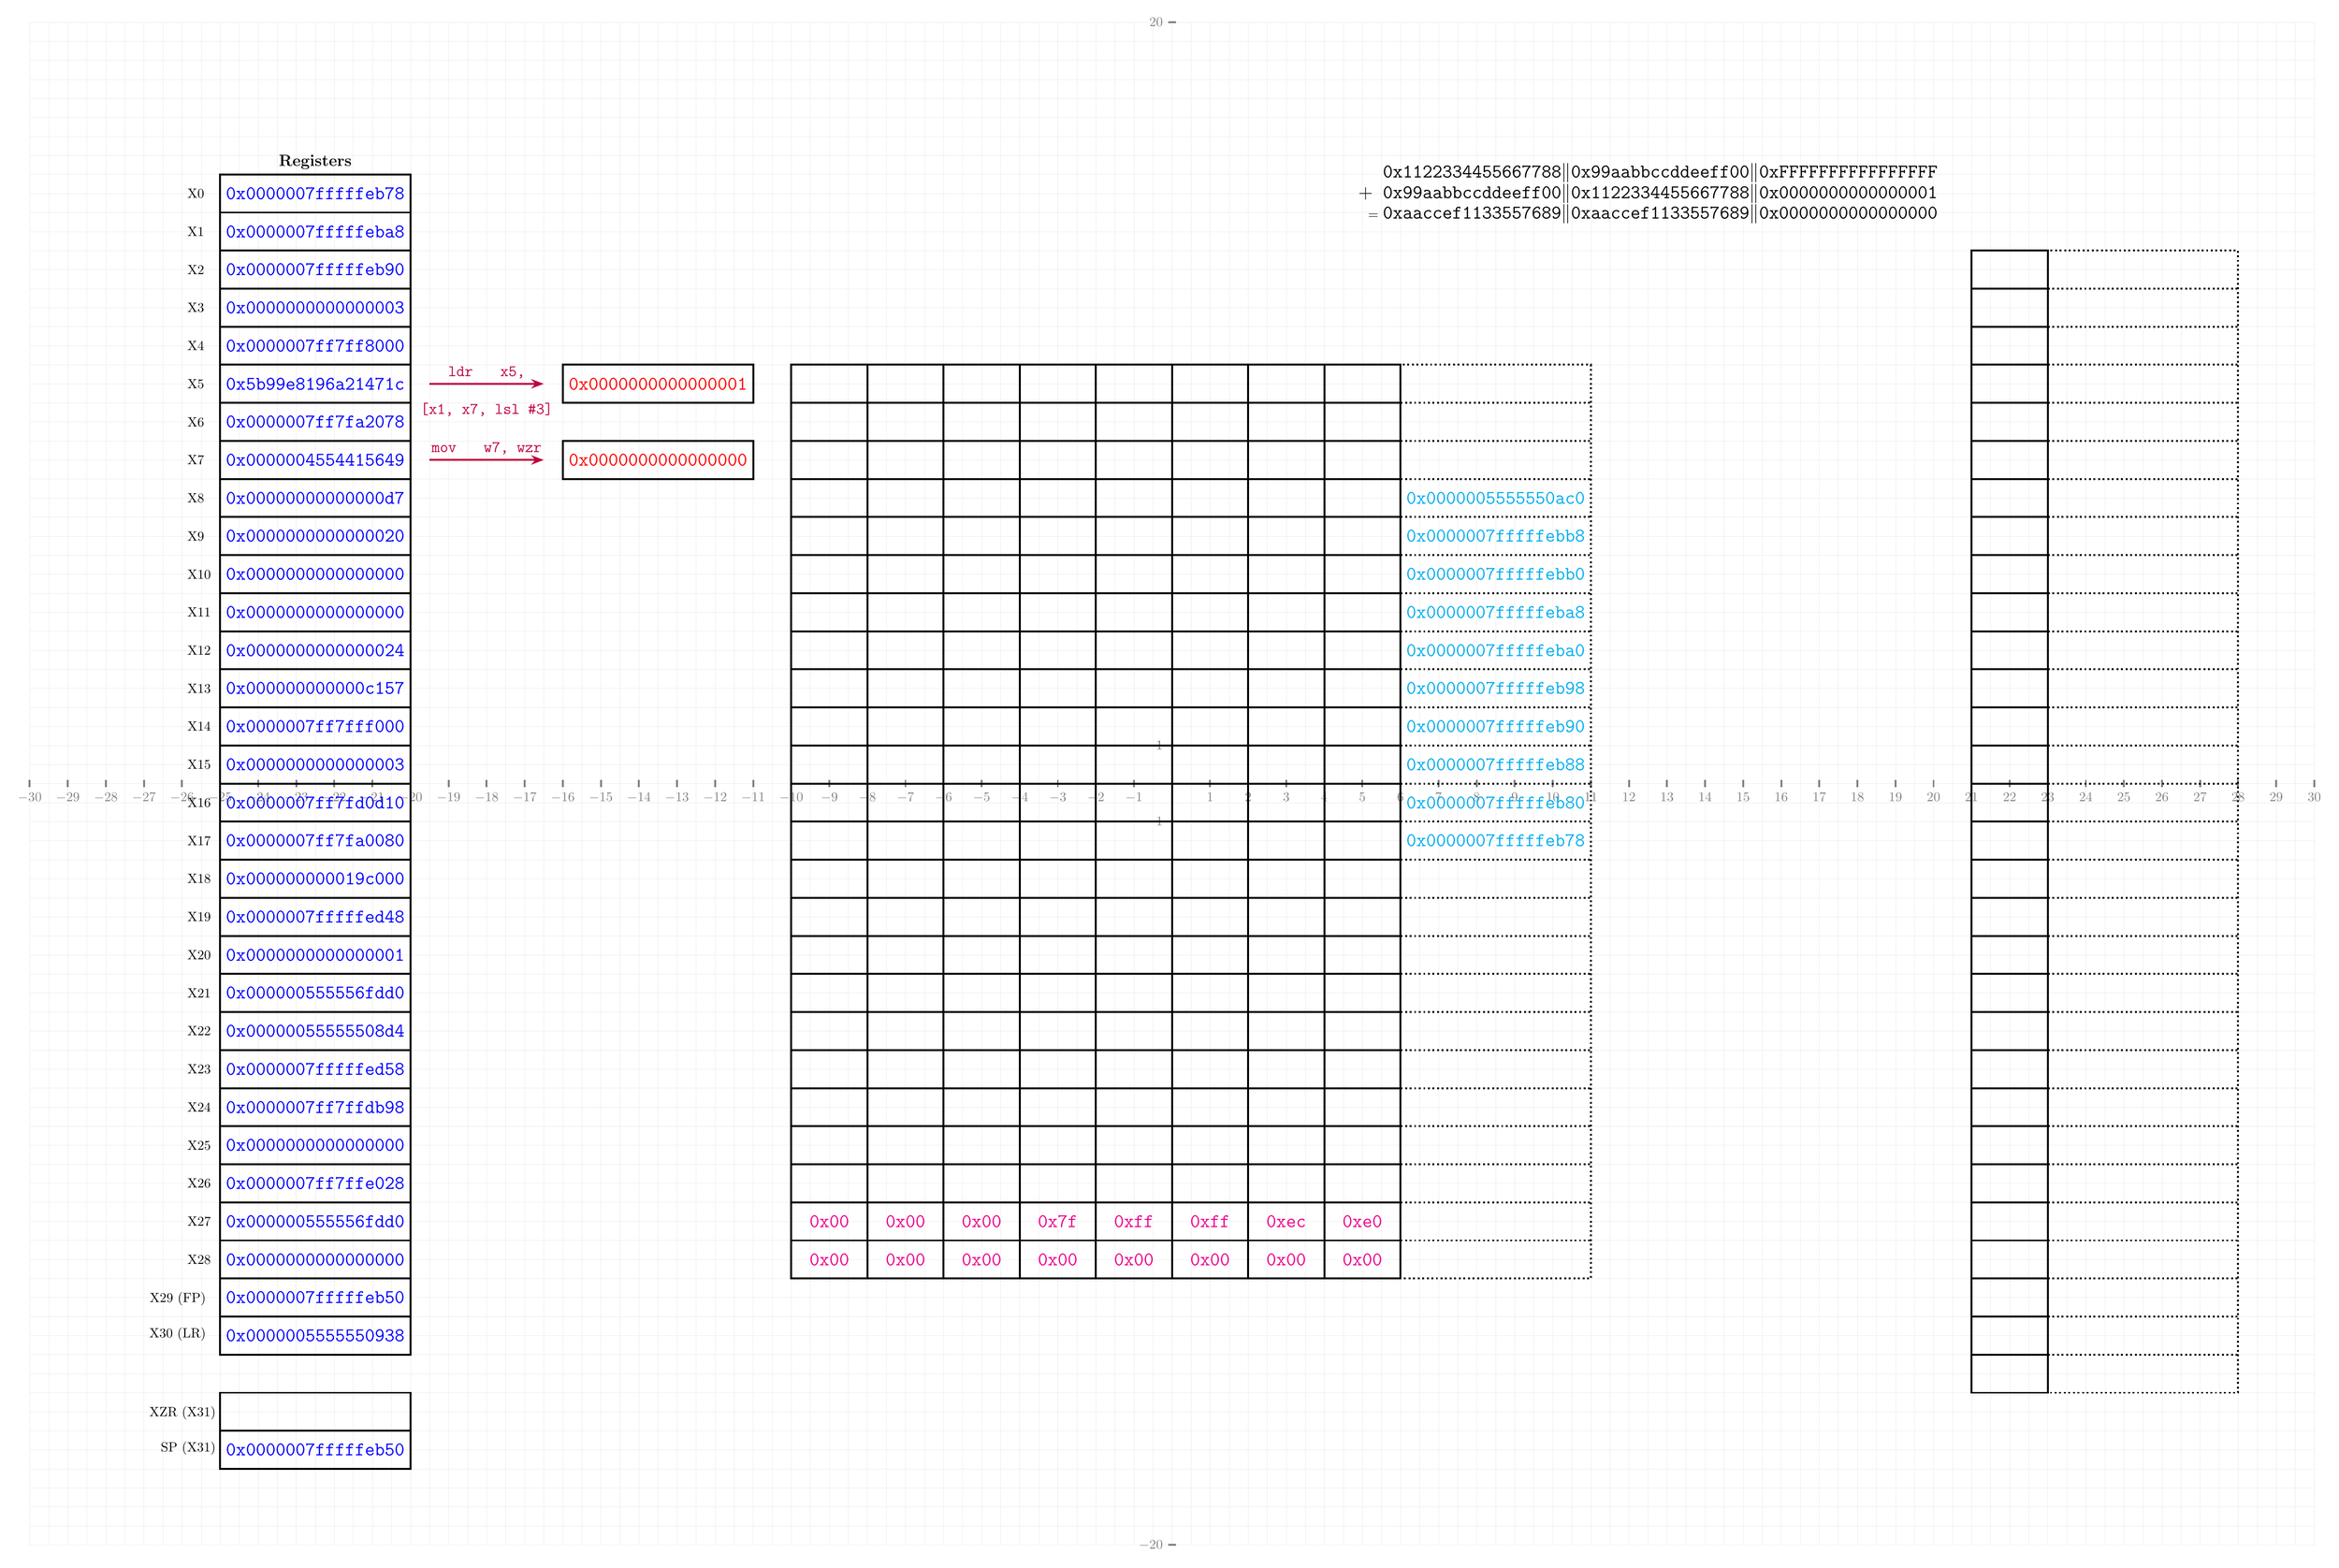
\begin{tikzpicture}[>=Stealth, line width=.5mm]
	\def \x{30}
	\def \y{20}
	\draw[very thin,color=gray!15,step=.5] (-\x,-\y) grid (\x,\y);
	
	\foreach \i in {-\x,...,-2,-1,1,2,...,\x}
	\draw[gray] (\i,.1)--(\i,-.1) node[below] {$\i$};%x-axis
	\foreach \i in {-\y,-1,1,1,\y}
	\draw[gray] (.1,\i)--(-.1,\i) node[left] {$\i$};%y-axis

%\begin{scope}[xshift=-7cm]
%	\draw[] (-10, -2) -- (-8, -3) -- (-8, -.5) -- (-8.5, 0) -- (-8, .5) -- (-8, 3) -- (-10, 2) -- cycle node[midway, right] {\Large\bf ALU};
%%	\draw[->, dashed, green!50!black, line width=1mm] (-10, 0) to (-10.5, 0) -- (-10.5, 18) -- (14, 18) -- (14, 14.5) -- (12, 14.5);
%	\draw[->] (-7, 2) to (-8, 2);
%	\draw[->] (-7, -2) to (-8, -2);
%\end{scope}
	
	\node[align=right] at (12.5,15.5) {\Large\ttfamily 0x1122334455667788$\parallel$0x99aabbccddeeff00$\parallel$0xFFFFFFFFFFFFFFFF\\
	\Large\ttfamily$+$\ 0x99aabbccddeeff00$\parallel$0x1122334455667788$\parallel$0x0000000000000001\\
	$=$\ \Large\ttfamily0xaaccef1133557689$\parallel$0xaaccef1133557689$\parallel$0x0000000000000000};

% Processor Core Section
\begin{scope}[xshift=-20cm]
	% Registers section (left side)
	\node[above] at (-2.5, 16) {\large\bf Registers};
	\draw[] (-5, -15) rectangle (0, 16); % Outer box
	\foreach \i in {0, 1, ..., 28} {
		\node[anchor=west] at (-6, 15.5-\i) {X\i};
	}
	\foreach \i in {15,14,...,-14} {
		\draw (-5,\i) -- (0, \i);
	}
	\node[anchor=west, align=flush right] at (-7, -14) {X29 (FP) \\[.5cm] X30 (LR)};

	\draw[] (-5, -18) rectangle (0, -16);
	\draw (-5,-17) -- (0, -17);
	\node[anchor=west, align=flush right] at (-7, -17) {XZR (X31) \\[.5cm]SP (X31)};
	
	\def\i{15.5}
	\foreach \j in {
		0x0000007fffffeb78, 0x0000007fffffeba8, 0x0000007fffffeb90,
		0x0000000000000003, 0x0000007ff7ff8000, 0x5b99e8196a21471c,
		0x0000007ff7fa2078, 0x0000004554415649, 0x00000000000000d7,
		0x0000000000000020, 0x0000000000000000, 0x0000000000000000,
		0x0000000000000024, 0x000000000000c157, 0x0000007ff7fff000,
		0x0000000000000003, 0x0000007ff7fd0d10, 0x0000007ff7fa0080,
		0x000000000019c000, 0x0000007fffffed48, 0x0000000000000001,
		0x000000555556fdd0, 0x00000055555508d4, 0x0000007fffffed58,
		0x0000007ff7ffdb98, 0x0000000000000000, 0x0000007ff7ffe028,
		0x000000555556fdd0, 0x0000000000000000, 0x0000007fffffeb50,
		0x0000005555550938  
	} {
		\node[blue] at (-2.5, \i) {\Large\texttt{\j}};
		\pgfmathsetmacro{\i}{\i- 1}
		\xdef\i{\i}
	}
	\node[blue] at (-2.5, -17.5) {\Large\texttt{0x0000007fffffeb50}};
\end{scope}

\begin{scope}[xshift=-11cm]
	% ldr     x5, [x1, x7, lsl #3]
	\draw[->, line width=.5mm, purple] (-8.5, 8.5) to (-5.5,8.5);
	\node[above] at (-7,8.5) {\color{purple}\large\ttfamily mov\hspace{.5cm} w7, wzr};
	\draw[] (-5, 8) rectangle (0, 9);
	\node[red] at (-2.5,8.5) {\Large\ttfamily 0x0000000000000000};
	
	% ldr     x5, [x1, x7, lsl #3]
	\draw[->, line width=.5mm, purple] (-8.5, 10.5) to (-5.5,10.5);
	\node[above,align=left] at (-7,10.5) {\color{purple}\large\ttfamily ldr\hspace{.5cm} x5,};
	\node[above,align=left] at (-7,9.5) {\color{purple}\large\ttfamily [x1, x7, lsl \#3]};
	\draw[] (-5, 10) rectangle (0, 11);
	\node[red] at (-2.5,10.5) {\Large\ttfamily 0x0000000000000001};
	
	% adr x15, y
%	\draw[->, line width=1mm] (-8.5, .5) to (-5.5,.5);
%	\node[above] at (-7,.5) {\color{purple}\large\ttfamily adr\hspace{.5cm} x15, y};
%	\draw[] (-5, 0) rectangle (0, 1);
%	
%	\node[red] at (-2.5,.5) {\Large\ttfamily 0x000000555557004c};
	
	% ldr x4, [x14]
%	\draw[->, line width=1mm] (-8.5, 11.5) to (-5.5,11.5);
%	\node[above] at (-7,11.5) {\color{purple}\large\ttfamily ldr\hspace{.5cm} x4, [x14]};
%	\draw[] (-5, 12) rectangle (0, 11);
%	
%	\node[teal] at (-2.5,11.5) {\Large\ttfamily 0x0000000800000005};
	
	% ldr x5, [x15]
%	\draw[->, line width=1mm] (-8.5, 10.5) to (-5.5,10.5);
%	\node[above] at (-7,10.5) {\color{purple}\large\ttfamily ldr\hspace{.5cm} x5, [x15]};
%	\draw[] (-5, 11) rectangle (0, 10);
%	
%	\node[orange] at (-2.5,10.5) {\Large\ttfamily 0x0000000000000008};
	
%	\draw[teal, ->, dashed, line width=1mm] (0, 11.5) -- (1, 11.5) -- (1, 17) -- (-18,17) -- (-18, 2) -- (-20, 2);
%	\draw[orange, ->, dashed, line width=1mm] (0, 10.5) -- (1.5, 10.5) -- (1.5, 17.5) -- (-17,17.5) -- (-17, -2) -- (-20, -2);
	
	% add x1, x4, x5
%	\draw[->, line width=1mm] (-8.5, 14.5) to (-5.5,14.5);
%	\node[above] at (-7,14.5) {\color{purple}\large\ttfamily add\hspace{.5cm} x1, x4, x5};
%	\draw[] (-5, 14) rectangle (0, 15);
	
%	\node[green!50!black] at (-2.5,14.5) {\Large\ttfamily 0x000000080000000d};
	
	% adr x0, fmt
%	\draw[->, line width=1mm] (-8.5, 15.5) to (-5.5,15.5);
%	\node[above] at (-7,15.5) {\color{purple}\large\ttfamily adr\hspace{.5cm} x0, fmt};
%	\draw[] (-5, 15) rectangle (0, 16);
%	
%	\node[red] at (-2.5,15.5) {\Large\ttfamily 0x0000005555570038};
\end{scope}
% Memory section (right side)
\begin{scope}[xshift=4cm]
	\draw[] (-14, -13) rectangle (2, 11); % Outer box
	\draw[dotted] (2, -13) rectangle (7, 11); % Outer box
	\foreach \i in {10,9,...,0,-1,-2,...,-12} {
		\draw (-14,\i) -- (2, \i);
	}
	\foreach \i in {-12,-10,...,0,2} {
		\draw (\i,-13) -- (\i, 11);
	}
	% Address
	\foreach \i in {10,9,...,0,-1,-2,...,-12} {
		\draw[dotted] (2,\i) -- (7, \i);
	}
%	\draw (0,14) to (0,14.5); \draw (2,14) to (2,15);
%	\draw[smooth] plot coordinates {(0,14.5) (.5, 15) (1.5, 14.5) (2,15)};
%	\draw (0,-17) to (0,-16); \draw (2,-16) to (2,-16.5);
%	\draw[smooth] plot coordinates {(2,-16.5) (1.5, -17) (.5, -16.5) (0,-17)};
	
	\def\i{1}
	\foreach \j in {
		0x00, 0x00, 0x00, 0x00, 0x00, 0x00, 0x00, 0x00
	} {
		\node[magenta] at (\i, -12.5) {\Large\texttt{\j}};
		\pgfmathsetmacro{\i}{\i-2}
		\xdef\i{\i}
	}
	\def\i{1}
	\foreach \j in {
		0xe0, 0xec, 0xff, 0xff, 0x7f, 0x00, 0x00, 0x00 
	} {
		\node[magenta] at (\i, -11.5) {\Large\texttt{\j}};
		\pgfmathsetmacro{\i}{\i-2}
		\xdef\i{\i}
	}
	
	\def\i{7.5}
	\foreach \j in {
		0x0000005555550ac0,
		0x0000007fffffebb8,
		0x0000007fffffebb0,
		0x0000007fffffeba8,
		0x0000007fffffeba0,
		0x0000007fffffeb98,
		0x0000007fffffeb90,
		0x0000007fffffeb88,
		0x0000007fffffeb80,
		0x0000007fffffeb78 
		} {
			\node[cyan] at (4.5, \i) {\Large\texttt{\j}};
			\pgfmathsetmacro{\i}{\i- 1}
			\xdef\i{\i}
		}

%	\def\i{-15.5}
%	\foreach \j in {
	%		0x54, 0x68, 0x65, 0x20,
	%		0x73, 0x75, 0x6d, 0x20,
	%		0x69, 0x73, 0x20, 0x25,
	%		0x64, 0x0a, 0x00, 0x00,
	%		0x05, 0x00, 0x00, 0x00,
	%		0x08, 0x00, 0x00, 0x00,
	%		0x00, 0x00, 0x00, 0x00,
	%		0x00, 0x00
	%	} {
	%		\node[magenta] at (1, \i) {\Large\texttt{\j}};
	%		\pgfmathsetmacro{\i}{\i+ 1}
	%		\xdef\i{\i}
	%	}
\end{scope}

\begin{scope}[xshift=21cm]
	% Contents
	\draw[] (0, -16) rectangle (2, 14); % Outer box
	\draw[dotted] (2, -16) rectangle (7, 14); % Outer box
	\foreach \i in {13,12,...,0,-1,-2,...,-15} {
		\draw (0,\i) -- (2, \i);
	}
	% Address
	\foreach \i in {13,12,...,0,-1,-2,...,-15} {
		\draw[dotted] (2,\i) -- (7, \i);
	}
%	\draw (0,14) to (0,14.5); \draw (2,14) to (2,15);
%	\draw[smooth] plot coordinates {(0,14.5) (.5, 15) (1.5, 14.5) (2,15)};
%	\draw (0,-17) to (0,-16); \draw (2,-16) to (2,-16.5);
%	\draw[smooth] plot coordinates {(2,-16.5) (1.5, -17) (.5, -16.5) (0,-17)};
	
%	\def\i{13.5}
%	\foreach \j in {
%		0x0000005555570055, 
%		0x0000005555570054, 
%		0x0000005555570053, 
%		0x0000005555570052, 
%		0x0000005555570051, 
%		0x0000005555570050, 
%		0x000000555557004f, 
%		0x000000555557004e,
%		0x000000555557004d, 
%		0x000000555557004c,
%		0x000000555557004b,
%		0x000000555557004a,
%		0x0000005555570049,
%		0x0000005555570048,
%		0x0000005555570047,
%		0x0000005555570046, 
%		0x0000005555570045,
%		0x0000005555570044,
%		0x0000005555570043,
%		0x0000005555570042,
%		0x0000005555570041,
%		0x0000005555570040,
%		0x0000005555570039,
%		0x0000005555570038,
%		0x0000005555570037,
%		0x0000005555570036,
%		0x0000005555570035,
%		0x0000005555570034,
%		0x0000005555570033,
%		0x0000005555570032
%	} {
%		\node[cyan] at (4.5, \i) {\Large\texttt{\j}};
%		\pgfmathsetmacro{\i}{\i- 1}
%		\xdef\i{\i}
%	}

%	\def\i{-15.5}
%	\foreach \j in {
%		0x54, 0x68, 0x65, 0x20,
%		0x73, 0x75, 0x6d, 0x20,
%		0x69, 0x73, 0x20, 0x25,
%		0x64, 0x0a, 0x00, 0x00,
%		0x05, 0x00, 0x00, 0x00,
%		0x08, 0x00, 0x00, 0x00,
%		0x00, 0x00, 0x00, 0x00,
%		0x00, 0x00
%	} {
%		\node[magenta] at (1, \i) {\Large\texttt{\j}};
%		\pgfmathsetmacro{\i}{\i+ 1}
%		\xdef\i{\i}
%	}
\end{scope}
\end{tikzpicture}
\end{document}
